\documentclass[11pt]{article}

\usepackage[margin=1in]{geometry}
\usepackage{amsmath,amssymb,amsthm}
\usepackage{mathtools}
\usepackage{bm}
\usepackage{tikz}
\usetikzlibrary{bayesnet,positioning,fit,shapes.geometric}
\pgfdeclarelayer{background}
\pgfsetlayers{background,main}
\usepackage{enumitem}
\usepackage{booktabs}
\usepackage{hyperref}

\title{A Graphical Model for Articulability:\\
\large Verifiable + Articulable + Taste, with pooled annotators}
\author{Notes for Alex's articulability project}
\date{\today}

\newcommand{\given}{\,|\,}
\newcommand{\E}{\mathbb{E}}
\newcommand{\Var}{\operatorname{Var}}
\newcommand{\indep}{\perp\!\!\!\perp}

\begin{document}
\maketitle

\section{Setting}

We have $n$ items indexed by $i$, with observed input $x_i$ (text) and observed quality
judgment $y_i \in \{0,1\}$ (or scalar). Judgments come from annotators indexed by $a$;
depending on the dataset we may or may not see annotator identities.

We posit $m$ \emph{metrics} (rubric criteria) indexed by $j \in \{1,\dots,m\}$. A metric is a
named, in principle articulable, dimension of quality (e.g.\ ``novelty'', ``statistical
rigor''). The metric set itself can be observed (provided rubric) or latent (extracted from
data). Metrics may be related hierarchically; let $\mathrm{pa}(j)$ denote the parents of
metric $j$ in a DAG (empty for flat models).

\section{Generative model}

For each metric $j$:
\begin{align}
r_j &\sim p(r) && \text{rubric statement (observed if provided)} \\
\text{ext}_j &\sim p(\text{ext} \given r_j) && \text{operationalization (regex / program / LLM judge)}
\end{align}

For each item $i$ and metric $j$:
\begin{align}
z_{i,j} &\sim p(z \given x_i, r_j, \{z_{i,k}\}_{k\in\mathrm{pa}(j)}) && \text{latent ``true'' value of metric $j$ on $x_i$} \\
\hat z_{i,j} &= \text{ext}_j(x_i) + \varepsilon^{\text{ext}}_{i,j} && \text{measurable proxy, noise } \sigma_j^2
\end{align}

For each annotator $a$ (in the most general case):
\begin{align}
b_a &\sim \mathcal{N}(\bar b, \tau_b^2) && \text{annotator threshold/intercept} \\
w_{a,j} &\sim \mathcal{N}(\bar w_j, \tau_{w,j}^2) && \text{personal weight on metric $j$} \\
\eta_{a,j}(\cdot) &\sim p(\eta \given r_j) && \text{personal reading of metric $j$ (link function)}
\end{align}

For each item $i$:
\begin{align}
s_i &\sim \mathcal{N}(0, \sigma_s^2) && \text{shared (community) inarticulable taste residual} \\
t_{i,a} &\sim \mathcal{N}(0, \sigma_t^2) && \text{personal inarticulable taste residual}
\end{align}

The judgment is generated by:
\begin{align}
\mu_{i,a} &= b_a \;+\; \sum_{j=1}^m w_{a,j}\,\eta_{a,j}(z_{i,j}) \;+\; s_i \;+\; t_{i,a} \\
y_{i,a} &\sim \text{Link}(\mu_{i,a}) && \text{e.g.\ Bernoulli}(\sigma(\mu_{i,a}))
\end{align}

When rationales are observed (e.g.\ peer review), we additionally have
\begin{align}
\rho_{i,a} &\sim p(\rho \given \{z_{i,j}\}_{j \in A_{i,a}}, \text{polarity}_{i,a,j})
\end{align}
where $A_{i,a}$ is the (latent) set of metrics annotator $a$ activated when judging $x_i$.

\paragraph{Decomposition into the three components.}
\[
\underbrace{y_{i,a}}_{\text{outcome}}
\;=\;
\underbrace{f(\hat z_{i,\cdot})}_{\text{verifiable}}
\;+\;
\underbrace{\sum_j w_{a,j}\bigl(\eta_{a,j}(z_{i,j}) - \hat z_{i,j}\bigr)}_{\text{articulable beyond verifiable}}
\;+\;
\underbrace{s_i + t_{i,a}}_{\text{taste}}
\]
The verifiable part uses only the cheap proxies $\hat z$. The articulable part adds the
information in $z$ that $\hat z$ misses (the verifiability gap, weighted by importance). The
taste part is the residual of human judgment that no metric---articulated or
latent---explains.

\section{Three regimes for annotator data}

We rarely observe individual annotator parameters cleanly. The model degrades gracefully
across three data regimes.

\subsection{Regime A: crossed (multi-annotator-per-item)}

Each item has multiple annotators, with overlap across items. \emph{Identification is
strongest here.} Examples in your portfolio: peer review (multiple reviewers per paper),
code review (sometimes multiple reviewers per PR).

Joint likelihood:
\[
p(\bm y \given x, \theta)
= \prod_{i,a} p\bigl(y_{i,a} \given x_i, b_a, w_{a,\cdot}, \eta_{a,\cdot}, s_i, t_{i,a}\bigr).
\]

Random-effects on annotators ($w_{a,j} \sim \mathcal{N}(\bar w_j, \tau_{w,j}^2)$) let us
estimate the population-mean weights $\bar w_j$ \emph{and} their dispersion $\tau_{w,j}^2$.
Cases where $\tau_{w,j}^2 \approx 0$ identify community-shared metrics; large
$\tau_{w,j}^2$ identifies metrics that mark personal preference.

\subsection{Regime B: pooled / mixture (annotator identities unknown)}

\emph{This is your most common case.} You see $y_i$ but not which annotator produced it,
or you see ``the community accepted this'' as an aggregated label. Examples: notice-and-
comment substantivity, creative-writing thread votes, joke-comment scores, patent
acceptance, homepage newsworthiness.

Two sub-cases:

\paragraph{B1. Latent-mixture pool.} A finite number $K$ of annotator types with mixing
weights $\bm\pi$. For each judgment we marginalize the type:
\[
p(y_i \given x_i)
= \sum_{k=1}^K \pi_k \cdot p\bigl(y_i \given x_i, b^{(k)}, w^{(k)}_{\cdot}, s_i\bigr).
\]
$K=1$ collapses to a single ``community annotator''; $K>1$ captures heterogeneity without
needing IDs. Identifiable via EM if there is enough variability in $x$ and the metric
loadings differ across types.

\paragraph{B2. Marginalized-population pool.} Treat each judgment as drawn from a fresh
annotator with parameters from the population:
\[
p(y_i \given x_i)
= \int p\bigl(y_i \given x_i, b, w, s_i\bigr)\,
        \mathcal{N}(b;\bar b,\tau_b^2)\,
        \prod_j \mathcal{N}(w_j;\bar w_j,\tau_{w,j}^2)
        \,dw\,db.
\]
With a logit link and Gaussian effects this is a standard random-effects logistic model;
$\bar w$ and $\tau_w$ are identifiable from variance in $y$ \emph{conditional on $\hat z$}.

In both pooled cases:
\begin{itemize}[topsep=2pt,itemsep=2pt]
  \item Personal taste $t_{i,a}$ and personal weight deviations $w_{a,j}-\bar w_j$ are
        \emph{not separately} identified---they collapse into a single dispersion
        parameter $\tau_{\text{pool}}$.
  \item Shared taste $s_i$ is still identified, because it varies systematically with $i$
        across all annotators (it is the part of $y$ predicted by $x$ \emph{after}
        regressing on $z$).
  \item The verifiability and articulability gaps remain identified (they are item-level
        quantities, not annotator-level).
\end{itemize}

\subsection{Regime C: single consensus label}

Only one $y_i$ per item, no annotator information at all (e.g.\ patent grant decisions,
many web-scraped labels). Equivalent to B2 with all annotator dispersion absorbed into
noise. The decomposition reduces to:
\[
y_i = f(\hat z_{i,\cdot}) + \sum_j \bar w_j\bigl(\eta_j(z_{i,j}) - \hat z_{i,j}\bigr) + s_i + \xi_i,
\]
where $\xi_i$ is irreducible noise that bundles annotator dispersion and personal taste.
Cannot distinguish ``community consensus residual'' $s_i$ from ``noise'' $\xi_i$ unless
you have repeated measurements per $x_i$ or an external proxy.

\section{The three gaps as restricted models}

Fit nested predictors and read off the lifts:
\begin{align}
\mathcal{M}_0:\quad &\hat y_i = \beta_0 \\
\mathcal{M}_1:\quad &\hat y_i = \beta_0 + f(\hat z_{i,\cdot}) && \text{verifiable only}\\
\mathcal{M}_2:\quad &\hat y_i = \beta_0 + \sum_j \bar w_j \,\eta_j(z_{i,j}) && \text{verifiable + articulable}\\
\mathcal{M}_3:\quad &\hat y_i = \text{dense}(x_i) && \text{everything (BT/regression on raw text)}
\end{align}
with metrics
\begin{align}
\text{Verifiability gap} &:= \text{AUC}(\mathcal{M}_2) - \text{AUC}(\mathcal{M}_1) \\
\text{Articulability gap} &:= \text{AUC}(\mathcal{M}_3) - \text{AUC}(\mathcal{M}_2) \\
\text{Taste residual variance} &:= \Var\bigl(y_i - \mathcal{M}_3(x_i)\bigr)
\end{align}
In Regime A, further split the taste residual into shared vs.\ personal by ICC of residuals
across annotators on the same item.

\section{Identification conditions}

\begin{enumerate}[topsep=2pt,itemsep=2pt]
\item Population means $\bar w_j$ and the verifiability gap require only $x_i, y_i$
      and a fixed set of $\hat z$ + LLM-judge $z$ predictions. \emph{Identifiable in all
      regimes.}
\item Annotator dispersion $\tau_{w,j}^2$ requires multiple judgments per item with
      systematic variation. \emph{Regime A only.}
\item Shared taste $s_i$ requires repeats or a sufficiently rich predictor space such
      that the dense model captures item-specific effects. \emph{Regimes A and B.}
\item Personal taste $t_{i,a}$ requires both crossed annotators \emph{and} sufficient
      coverage that we can attribute residuals to individuals. \emph{Regime A only.}
\item Hierarchical structure on metrics (DAG via $\mathrm{pa}(j)$) requires either an
      observed rubric tree or extracted entailment relations between $z_j$'s.
\end{enumerate}

A quick heuristic: \emph{which questions can each dataset answer?}

\begin{center}
\small
\begin{tabular}{lcccc}
\toprule
Dataset & V-gap & A-gap & Shared taste $s_i$ & Personal taste $t_{i,a}$ \\
\midrule
Peer review (multi-reviewer + rationales) & \checkmark & \checkmark & \checkmark & \checkmark \\
Code review (multiple reviewers per PR)   & \checkmark & \checkmark & \checkmark & partial \\
Notice \& comment (pooled)                 & \checkmark & \checkmark & \checkmark & --- \\
Creative writing (Reddit votes, pooled)    & \checkmark & \checkmark & partial    & --- \\
Humor (joke score, pooled)                 & \checkmark & \checkmark & partial    & --- \\
Patents (single decision)                  & \checkmark & \checkmark & ---        & --- \\
Press releases (single label)              & \checkmark & \checkmark & ---        & --- \\
Newsworthiness (homepage, pooled)          & \checkmark & \checkmark & partial    & --- \\
Math (verifier ground truth)               & \checkmark & ---       & ---        & --- \\
\bottomrule
\end{tabular}
\end{center}

\section{Choice of aggregation function}

Linear-in-metrics (above) is convenient but is wrong in three common cases:

\begin{enumerate}[topsep=2pt,itemsep=2pt]
\item \textbf{Dealbreakers / vetoes.} A single fatal flaw rejects regardless of others
      (peer review, patents). Use noisy-AND on dealbreaker metrics or a min-pooling layer:
      $\mu = \min_{j \in D} z_{i,j} + \sum_{j\notin D} w_j z_{i,j}$.
\item \textbf{Threshold effects.} Quality jumps once a criterion crosses a level (humor,
      newsworthiness). Replace $z$ with $\mathbb{1}\{z > \theta_j\}$ before weighting.
\item \textbf{Substitutability.} Multiple ways to be good (creative writing: dense plot
      \emph{or} strong voice). Use a softmax / log-sum-exp over substitutable metric
      bundles instead of a sum.
\end{enumerate}

These are local refinements; the rest of the framework (gaps, identification) is unchanged.

\section{Plate diagram}

\begin{center}
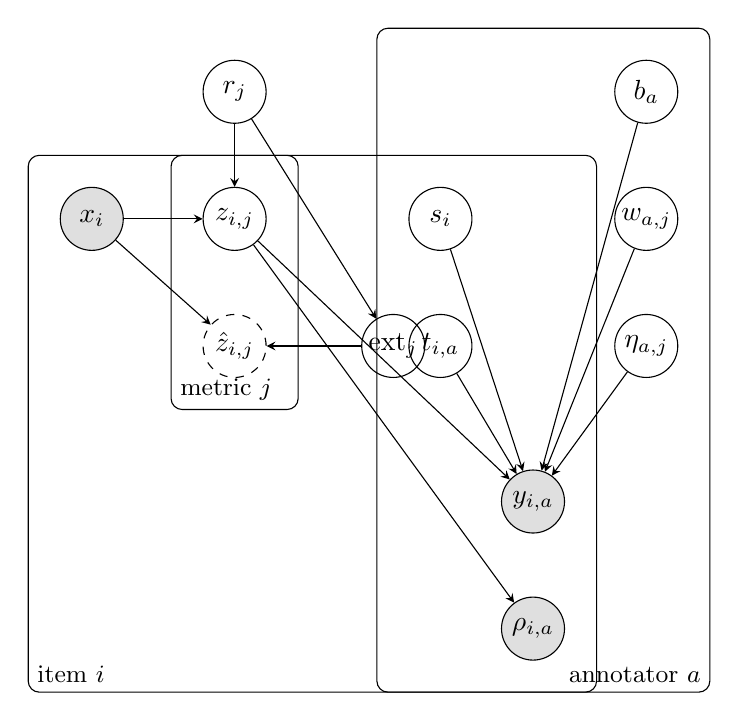
\begin{tikzpicture}[
  obs/.style={circle, draw, fill=gray!25, minimum size=8mm, inner sep=1pt},
  lat/.style={circle, draw, minimum size=8mm, inner sep=1pt},
  det/.style={circle, draw, dashed, minimum size=8mm, inner sep=1pt},
  plate/.style={draw, rectangle, rounded corners, inner sep=4mm},
  every label/.style={font=\small},
  >=stealth
]

\node[obs] (x) {$x_i$};
\node[lat, right=10mm of x] (z) {$z_{i,j}$};
\node[det, below=8mm of z] (zhat) {$\hat z_{i,j}$};
\node[lat, above=8mm of z] (r) {$r_j$};
\node[lat, above=8mm of zhat, right=12mm of zhat] (ext) {$\text{ext}_j$};

\node[lat, right=18mm of z] (s) {$s_i$};
\node[lat, below=8mm of s] (t) {$t_{i,a}$};

\node[lat, right=18mm of s] (w) {$w_{a,j}$};
\node[lat, above=8mm of w] (b) {$b_a$};
\node[lat, below=8mm of w] (eta) {$\eta_{a,j}$};

\node[obs, below right=14mm and 6mm of t] (y) {$y_{i,a}$};
\node[obs, below=8mm of y] (rho) {$\rho_{i,a}$};

\draw[->] (x) -- (z);
\draw[->] (r) -- (z);
\draw[->] (r) -- (ext);
\draw[->] (ext) -- (zhat);
\draw[->] (x) -- (zhat);
\draw[->] (z) -- (y);
\draw[->] (s) -- (y);
\draw[->] (t) -- (y);
\draw[->] (w) -- (y);
\draw[->] (b) -- (y);
\draw[->] (eta) -- (y);
\draw[->] (z) -- (rho);

\begin{pgfonlayer}{background}
  \node[plate, fit=(z)(zhat), label={[anchor=south west]south west:metric $j$}] (Pj) {};
  \node[plate, fit=(x)(z)(zhat)(s)(t)(y)(rho), label={[anchor=south west]south west:item $i$}] (Pi) {};
  \node[plate, fit=(b)(w)(eta)(t)(y)(rho), label={[anchor=south east]south east:annotator $a$}] (Pa) {};
\end{pgfonlayer}

\end{tikzpicture}
\end{center}

\noindent
Shaded = observed; solid circle = latent; dashed = deterministic given parents. The
annotator plate collapses to a single node in Regime C and to a marginalized random
effect in Regime B.

\section{Connection to your existing apparatus}

\begin{itemize}[topsep=2pt,itemsep=2pt]
\item \textbf{Verifier-first programs} populate $\hat z_{\cdot,j}$ where $\text{ext}_j$ is
      a synthesized program. Library convergence rate is your direct estimate of
      $\dim(\hat z)$ for the task.
\item \textbf{STaR / $z_+, z_-$ extraction} produces samples from
      $p(\rho_{i,a} \given z_{i,A_{i,a}}, \text{polarity})$, which is partial observation
      of the latent metric activations $A_{i,a}$.
\item \textbf{Haupt entailment hierarchy} estimates the $\mathrm{pa}(\cdot)$ DAG from the
      $z$'s, allowing you to fit the hierarchical version of the model rather than the
      flat one.
\item \textbf{Thin/thick classification} per metric is the empirical question of whether
      $\Var(\hat z_{i,j} - z_{i,j}) \approx 0$ when $\text{ext}_j$ is a program (thin) or
      requires an LLM (thick).
\end{itemize}

\section{Open questions}

\begin{enumerate}[topsep=2pt,itemsep=2pt]
\item Is $z_{i,j}$ a platonic latent (realist) or a community fixed-point (constructive)?
      Affects whether the model is generative or only descriptive.
\item In pooled regimes, does $K{=}1$ vs.\ $K{>}1$ in mixture pooling actually buy you
      anything, or does the population-effects formulation suffice?
\item Should aggregation be per-task (peer review uses dealbreakers; humor uses
      thresholds; creative writing uses substitution)? Probably yes; build a small library
      of aggregators and pick by held-out fit.
\item How do we handle the case where the rubric statement $r_j$ is itself uncertain
      (extracted from text, not given)? Treat $r_j$ as latent and infer with
      Dirichlet-process or fixed-vocabulary priors over rubric items.
\end{enumerate}

\end{document}
